\begin{center}
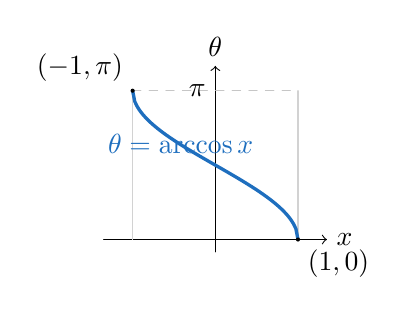
\begin{tikzpicture}[scale=1.05, line cap=round, line join=round]
  \definecolor{trigblue}{RGB}{30,110,190}
  \draw[->] (-1.35,0)--(1.35,0) node[right] {$x$};
  \draw[->] (0,-0.15)--(0,2.1) node[above] {$\theta$};
  \draw[gray!35] (-1,0)--(-1,1.8);
  \draw[gray!35] (1,0)--(1,1.8);
  \draw[gray!45,dashed] (-1,1.8)--(1,1.8);
  \draw[very thick,trigblue,domain=-1:1,samples=80]
    plot ({\x},{1.8*acos(\x)/180});
  \fill (-1,1.8) circle (0.025) node[above left] {$(-1,\pi)$};
  \fill (1,0) circle (0.025) node[below right] {$(1,0)$};
  \node[trigblue] at (-0.42,1.16) {$\theta=\arccos x$};
  \node[left] at (0,1.8) {$\pi$};
\end{tikzpicture}
\end{center}


\begin{definitionbox}{Definition}
\begin{definition}[Inverse cosine]
\label{def:inverse-cosine}
The \emph{inverse cosine} function is the inverse of cosine after cosine is
restricted to the interval $[0,\pi]$. It is denoted by $\arccos$ or
$\cos^{-1}$ and has domain $[-1,1]$ and range $[0,\pi]$.
\[
  \arccos x=\theta
  \quad\Longleftrightarrow\quad
  \cos\theta=x
  \quad\text{and}\quad
  0\leq\theta\leq\pi.
\]
\end{definition}
\end{definitionbox}
\begin{remark*}[Standard quantified statement]
For every admissible input satisfying the hypotheses of the statement, the
displayed definition or assertion holds in the stated domain.
\end{remark*}

\begin{remark*}[Interpretation]
The statement records the named trigonometric object or identity together with
its intended domain of use.
\end{remark*}

\begin{remark*}[Domain and range]
The full cosine function has domain all real-valued angle measures and range
$[-1,1]$. The inverse cosine function reverses the restricted cosine function,
so its domain is $[-1,1]$ and its range is the principal interval $[0,\pi]$.
\end{remark*}
\begin{dependencies}
\begin{itemize}
  \item \hyperref[def:unit-circle-cosine]{Unit-circle cosine}
  \item \hyperref[def:radian-measure]{Radian measure}
\end{itemize}
\end{dependencies}

\begin{theorembox}{Theorem}
\begin{theorem}[Principal inverse cosine identities]
\label{thm:inverse-cosine-identities}
For every $x\in[-1,1]$,
\[
  \cos(\arccos x)=x.
\]
For every $\theta\in[0,\pi]$,
\[
  \arccos(\cos\theta)=\theta.
\]
\end{theorem}
\end{theorembox}
\begin{remark*}[Interpretation]
The statement records the named trigonometric object or identity together with
its intended domain of use.
\end{remark*}

\begin{remark*}[Standard quantified statement]
$\forall x\in[-1,1]$, $\cos(\arccos x)=x$, and
$\forall \theta\in[0,\pi]$, $\arccos(\cos\theta)=\theta$.
\end{remark*}
\begin{dependencies}
\begin{itemize}
  \item \hyperref[def:inverse-cosine]{Inverse cosine}
\end{itemize}
\end{dependencies}
